\documentclass[a4paper]{article}
\usepackage{fullpage}
\usepackage{graphicx}
\title{MageComet}
\author{Vincent Xue}
\date{\today}
\begin{document}
\maketitle
\section{Purpose}
MageComet is a web application designed for quick annotation and manipulation of MAGE-TAB files. The webapp features tools that allow curators to easily edit MAGE-TAB documents, without spending excessive time and effort formating files to MAGE-TAB specifications. MageComet's goal is to reduce the amount of time editing MAGE-TAB documents by automating tasks commonly encountered during curation. This automation allows curators to focus more on the biological data presented instead of spending time formating the document.

\section{Loading Files}
There are two ways to begin editing a set of MAGE-TAB files.
\subsubsection*{Direct Loading}
Direct loading is used when MAGE-TAB documents are locally stored on the client machine. There are two files required to proceed, namely the the SDRF, and IDF files which are usually appended by "sdrf.txt" and "idf.txt" respectively. Though the MAGE-TAB specification does not mandate that SDRF and IDF files have these suffixes, MageComet uses these suffixes during load, and will not proceed without them.

When starting the MageComet webapp, the user will be presented with the "Load Tab". This can be seen in Figure \ref{initial}.

\begin{figure}[h]
\caption{The opening load tab}
\centering
\label{initial}
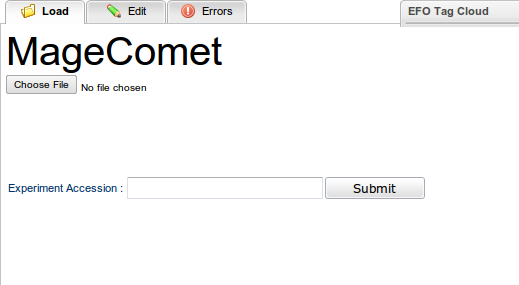
\includegraphics[width=10cm]{images/Load}
\end{figure}

To load the MAGE-TAB files to the server, the user must click the "Choose File" button. A popup will appear and the user can select either the SDRF file or the IDF file to upload first. The same "Choose File" button must be clicked after the first file has loaded. When both files have successfully been loaded, the screen should like like Figure \ref{load2}.

\begin{figure}[h]
\caption{Snapshot after loading IDF and SDRF files}
\centering
\label{load2}
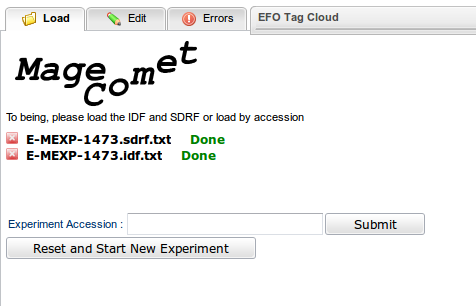
\includegraphics[width=10cm]{images/Load2}
\end{figure}

\subsubsection*{ArrayExpress FTP}
To load a file via the ArrayExpress FTP service the user can use the form directly below the "Choose File" button. The user can simply type in the experiment accession and click submit, which will automatically fetch and load the IDF and SDRF files.

\section{Filtering Data}
Once the files have been loaded the user can proceed to the "Edit" tab. If loading has been successful, the page should resemble Figure \ref{edittab}.

\begin{figure}[h]
\caption{Edit after successful load}
\centering
\label{edittab}
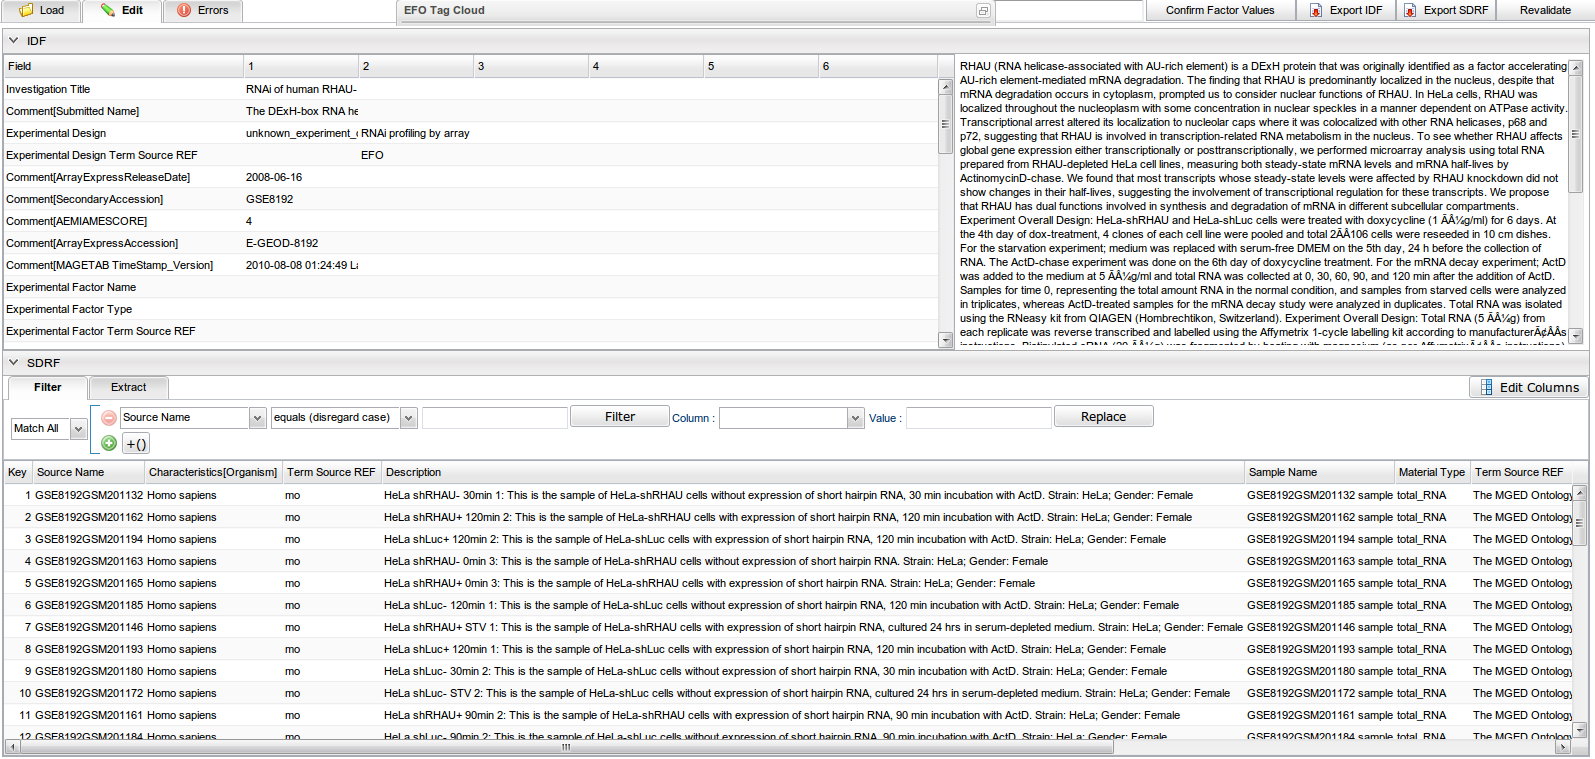
\includegraphics[width=16cm]{images/Edit}
\end{figure}

The first tool that is visible to the user is the filter and replace tool as shown in Figure \ref{filterandreplace}. This tool is very similar to the search and replace tool in excel, but it is designed to be more specific for editing columns of data.

There are 5 components of this tool that a user can customize.
\begin{enumerate}
\item[\bf{A}] Filter Column - This is the column that has a trait of interest. Usually this is the "Description" column.
\item[\bf{B}] Logic - This dropdown box determines the logic a user wants to apply on the filter column It contains a list of items such "equals", "contains", "does not contain" and more.
\item[\bf{C}] Filter Value - This is the value the user will filter on.
\end{enumerate}
Parts A, B, and C contain the logic for filtering. 

Example: A user wants to filter for all the rows that contain female in the description column. The values for the A, B, and C would be A:Description, B:Contains, C:Female

\begin{enumerate}
\item[\bf{D}] Target Column - The column whose value will be set
\item[\bf{E}] New Value - The value that the target column will be set to.
\end{enumerate}
Parts D and E contain the logic for replacing.

Example: A user wants to replace all the values in the column Characteristics[sex] with female. The values for D and E would be D:Characteristic[sex], E:female.

\bf{Note: The value for D must be a column that already exists}\rm

\begin{figure}[h]
\caption{Filter and Replace}
\centering
\label{filterandreplace}
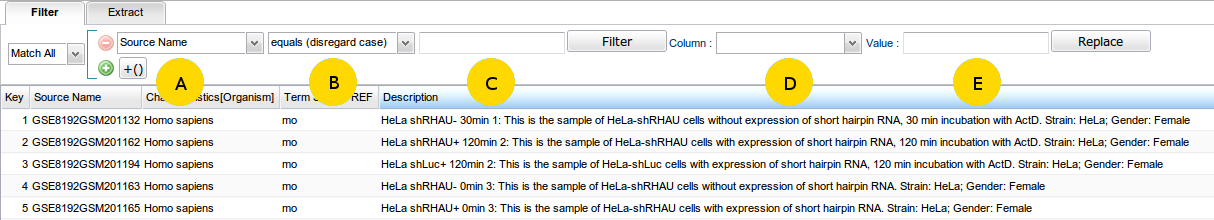
\includegraphics[width=17cm]{images/Filter}
\end{figure}
\section{Column Manipulation}
All column manipulation must be performed from the "Column Editor". The button to activate this editor is shown in Figure \ref{columneditbutton} and the popup editor is shown in Figure \ref{columneditor}. 

In this column editor, all of the rows are represented as rows. The left side of the editor designated by \bf{A}\rm~ is the clipboard. This section of the popup acts as a scratch buffer where columns are discarded to. In addition, new columns also appear in this clipboard before they are placed. 

The right side of the editor designated by \bf{C}\rm ~is the representation of the SDRF columns. This section shows what columns are in the SDRF and in what order it appears.

\begin{figure}[h]
\caption{Column editor button}
\centering
\label{columneditbutton}
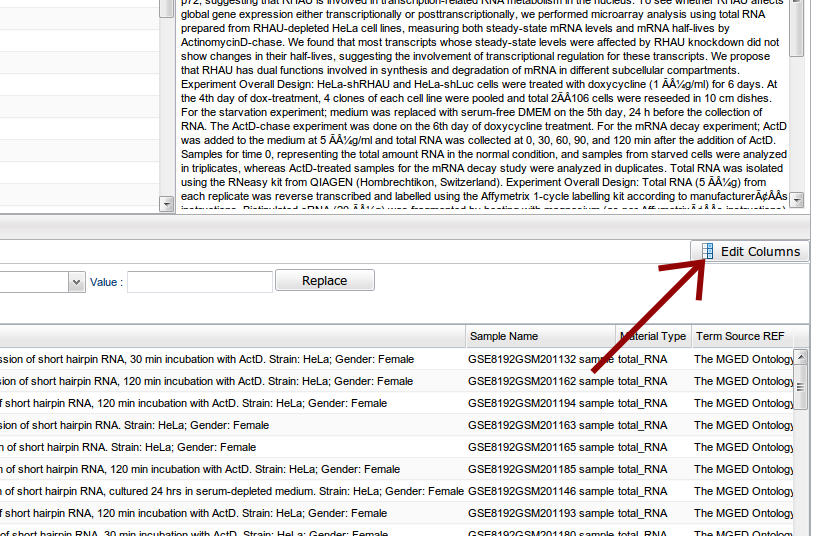
\includegraphics[width=10cm]{images/ColumnEditor}
\end{figure}

\begin{figure}[h]
\caption{Column editor}
\centering
\label{columneditor}
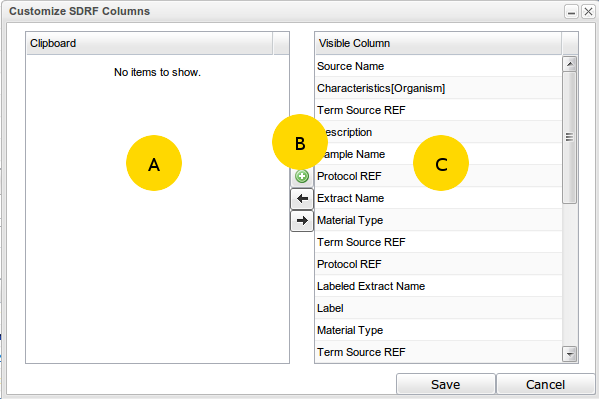
\includegraphics[width=10cm]{images/ceditor}
\end{figure}
\newpage
\subsubsection*{Adding Columns}
To add a column, click the green plus sign below \bf{B}\rm. This will add a row to the clipboard \bf{A}\rm.
\subsubsection*{Removing Columns}
To remove a column, drag the desired column from section \bf{C}\rm~ to section \bf{A}\rm. In addition, a user can also select the column from section \bf{C}\rm~ and click the $\leftarrow$ button.
\subsubsection*{Reordering Columns}
To reorder column orders, drag and drop the row to the desired position.
\subsubsection*{Renaming Columns}
To rename a column, double click the row.
\section{Extracting Data}
The extract tool is a feature that splits row values formated with delimiters. If all of the rows in a column are formated similarly, this tool allows the user to separate a single column into many. An example of splittable column is seen in Figure \ref{splittable}. 

\begin{figure}[h]
\caption{Example of a splittable column}
\centering
\label{splittable}
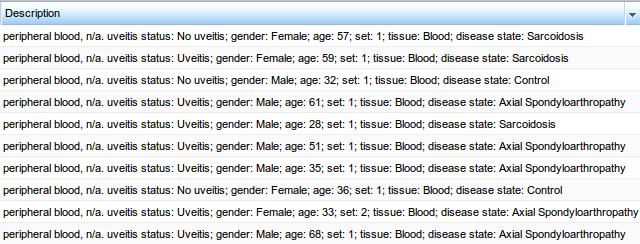
\includegraphics[width=15cm]{images/splittable}
\end{figure}

In this example the "Description" column should be separated into new columns for organism part, disease stage, sex, age, set, and disease state. Automatic splitting is difficult and avoided because a single column could have many different combinations of delimiters. In this example alone, there are commas, semicolons, colons, and text delimiters in a single row. However, because this format is consistent throughout the column, the extract feature implemented in MageComet works well in these situations.

\newpage
The extract tool is located in the same panel as the filter tool. By clicking on the "Extract" tab, the user can activate the panel that should resemble Figure \ref{extracttool}. Like the filter tool, the extract tool has 5 components which the user must fill in.



\begin{enumerate}
\item[\bf{A}] From Column - This is the column that is splittable. Usually this is the "Description" column.
\item[\bf{B}] Left Input -  This field should be filled in with the text that is left of the value that should be extracted. The input however should be \bf{unique}\rm~ as it will only match the first input found.
\item[\bf{C}] Right Input - This field should be filled in with the text that is right of the value that should be extracted.
\item[\bf{D}] Type Column - This field is the target column type. The possible choices are "Clipboard", "Characteristic", Factor Value", or "Both".
\item[\bf{E}] Column Name- This field is the target column name. This is the value that will fit in between the brackets [~].
\end{enumerate}

\begin{figure}[h]
\caption{Extract}
\centering
\label{extracttool}
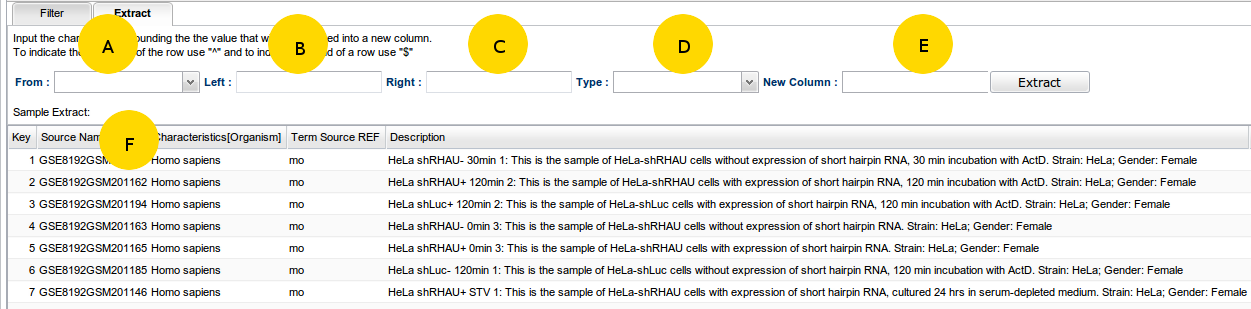
\includegraphics[width=17cm]{images/Extract}
\end{figure}
When the user completes values for \bf{B}\rm ~and \bf{C}\rm , the section designated by \bf{F}\rm~ will show the sample values that will be extracted. 

\subsubsection*{More Examples}

The following lists the input values for \bf{B}\rm ~and \bf{C}\rm~ that will extract the targeted value successfully for Figure \ref{splittable}.
\begin{table}
\begin{center}
\begin{tabular}{| c c r |}
\hline
Left & Right & Sample Extract Row 1\\
\hline
  $\mathbin{\char`\^}$ & , & peripheral blood \\
\hline
status: & ; & No uveitis \\
\hline
gender: & ; & Female \\
\hline
set: & ; & 1 \\
\hline
tissue: & ; & Blood \\
\hline
state: & $\$$ & Sarcoidosis\\
\hline
\end{tabular}
\end{center}
\caption{Sample inputs and outputs for Figure \ref{splittable}}
\end{table}

\newpage
The following lists the input values for \bf{B}\rm ~and \bf{C}\rm~ that will extract the targeted value successfully for Figure \ref{splittable2}.

\begin{figure}[h]
\caption{Another example of a splittable column (intermediate difficulty)}
\centering
\label{splittable2}
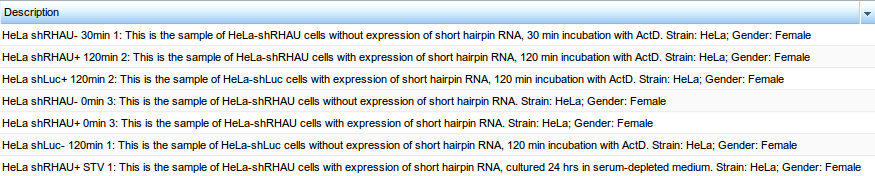
\includegraphics[width=17cm]{images/moreextract}
\end{figure}


\begin{table}[h]
\begin{center}
\begin{tabular}{| c c r |}
\hline
Left & Right & Sample Extract Row 1\\
\hline
  $\mathbin{\char`\^}$ & [0-9] & HeLa shRHAU-\\
\hline
[+-] & min & 30 \\
\hline
gender: & ; & Female \\
\hline
RNA, & min & 30 \\
\hline
Strain: & ; & HeLa \\
\hline
Gender: & $\$$ & Female\\
\hline
\end{tabular}
\end{center}
\caption{Sample inputs and outputs for Figure \ref{splittable2}}
\end{table}





\section{Tag Cloud}
The tag cloud is a feature that helps curators identify important biological information text-mined from the IDF and SDRF text. To open the window, click on the button designated by Figure \ref{tagcloudopen}. A window should pop up that resembles Figure \ref{tagcloud}. 

\begin{figure}[h]
\caption{Default tagcloud position}
\centering
\label{tagcloudopen}
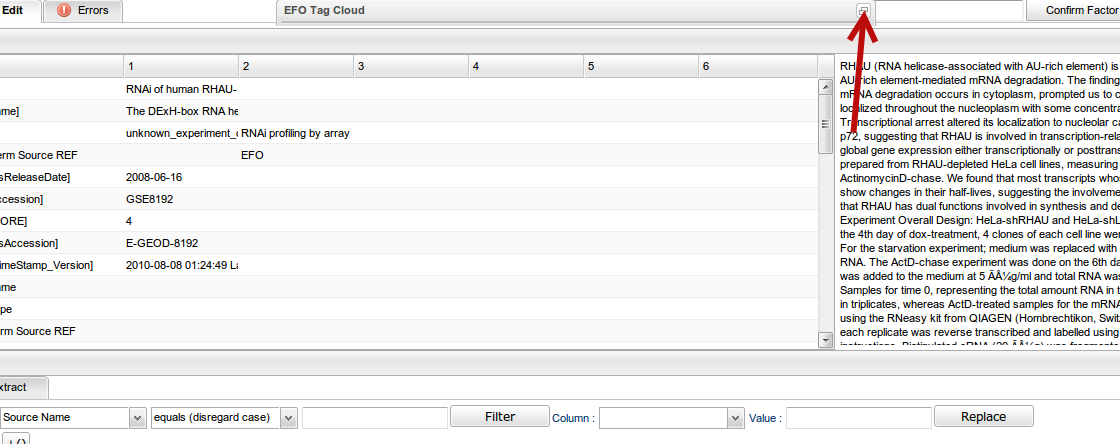
\includegraphics[width=17cm]{images/tagcloudopen}
\end{figure}

\begin{figure}[h]
\caption{The TagCloud Window}
\centering
\label{tagcloud}
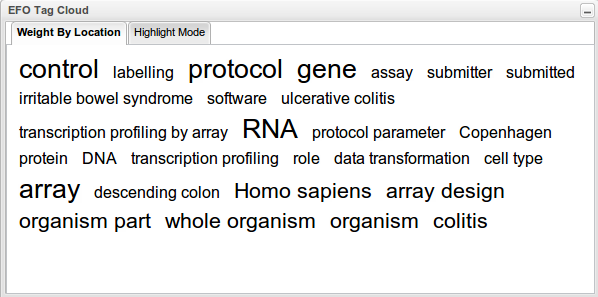
\includegraphics[width=12cm]{images/tagcloud}
\end{figure}

In the tagcloud representation of the text, each item represents an EFO ontology term that has been mined from 2 documents. The size of an item corresponds to where the term came from. The smallest size, indicates that only the IDF mentions the word. The medium sized text indicates that the text was mined from the SDRF, and the largest sized text indicates that both the IDF and SDRF mention the ontology term. 

\subsubsection*{Adding characteristics via tagcloud}
A sub feature of the tag cloud is the ability to add a characteristic term to all rows in a document. This feature is useful when some vital information is mentioned in the experiment description but is not mentioned in the SDRF document. By clicking on the term in the tag cloud, a new popup will show up, giving the user the option of adding the selected term to the SDRF. Figure \ref{tagcloudsubfeature}.

When a tag cloud item is clicked, a popup will appear, providing some useful information about the term. It usually provides a description near the top, which is pulled from the EFO ontology and the term source number.

The user can choose to add a characteristic column, term source ref column, or a term source number column to the SDRF, depending on how granular the curation is. The input field designated by \bf{A}\rm~ in Figure \ref{tagcloudsubfeature} is the value that will be placed in the brackets [~].


\begin{figure}[h]
\caption{Adding a characteristic via tagcloud}
\centering
\label{tagcloudsubfeature}
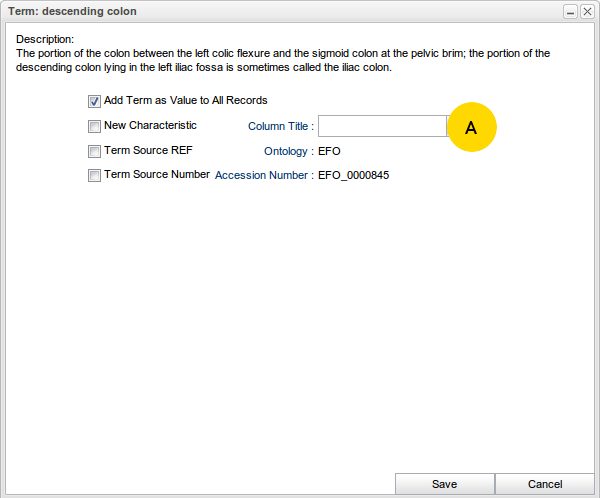
\includegraphics[width=12cm]{images/tagcloud_subfeature}
\end{figure}

\newpage
\subsubsection*{Highlighting text via tagcloud}
Another sub feature of the tag cloud is to highlight text. This feature can be accessed by clicking the "Highlight Mode" tab in Figure \ref{tagcloud}. The same cloud will appear, but clicking on a term will cause it to highlight on the page. This is demonstrated by Figure \ref{highlight}.

\begin{figure}[h]
\caption{Tagcloud highlight feature}
\centering
\label{highlight}
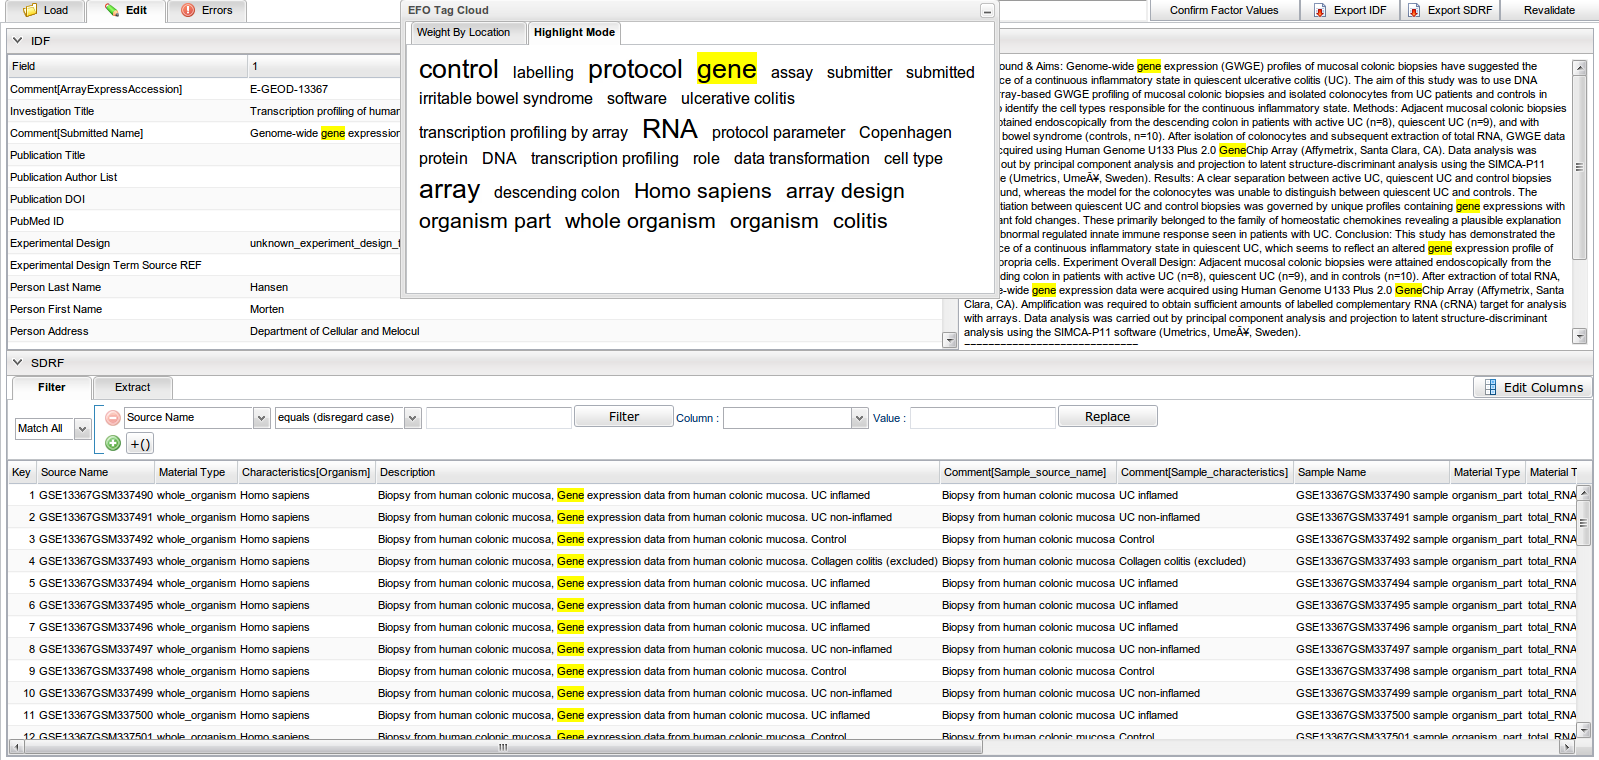
\includegraphics[width=17cm]{images/highlight}
\end{figure}

\newpage
\section{EFO Search Box}
The EFO search box is a convenience feature implemented into MageComet. If the user wants to confirm that an EFO term exists in the EFO ontology, the EFO search box can be used as shown in Figure \ref{searchbox}.

The search field autocompletes based on the query text and displays 3 terms that match the query. If an item is in parentheses as shown with human, the value in parentheses is the standard name for the synonym found. If the user wants to copy the standard ontology name, pressing enter while over the term will fill in the field, making it copyable.

\begin{figure}[h]
\caption{EFO searchbox}
\centering
\label{searchbox}
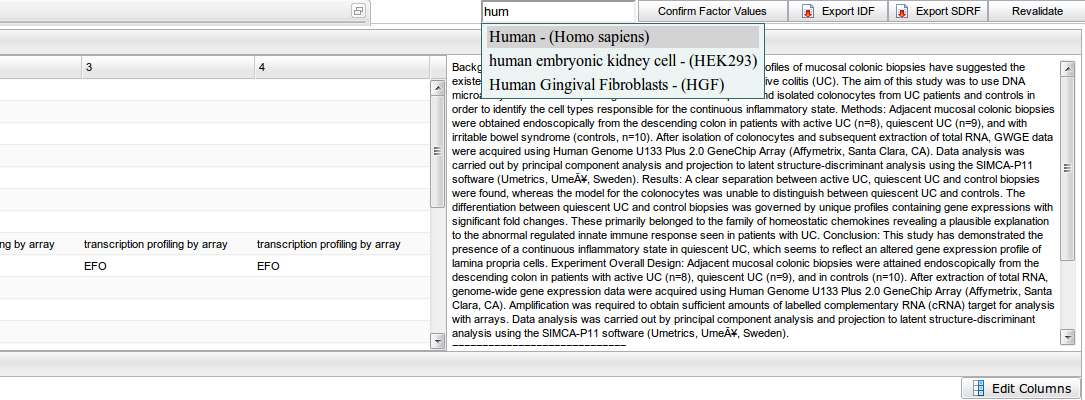
\includegraphics[width=17cm]{images/searchbox}
\end{figure}



\section{Adding Factor Values}
When the user has finished extracting the factor values in the SDRF document, the IDF document must be updated to reflect the changes. The IDF document can be updated via the "Confirm Factor Value" button as shown in Figure \ref{confirmfactorbutton}.

Once clicked a window will appear that shows all of the Factor Values in the SDRF. Figure \ref{confirmfactorvalue}. After filling in the corresponding Factor Value Types and clicking save, the IDF document will have the correct values automatically inserted.




\begin{figure}[h]
\caption{Confirm factor value button}
\centering
\label{confirmfactorbutton}
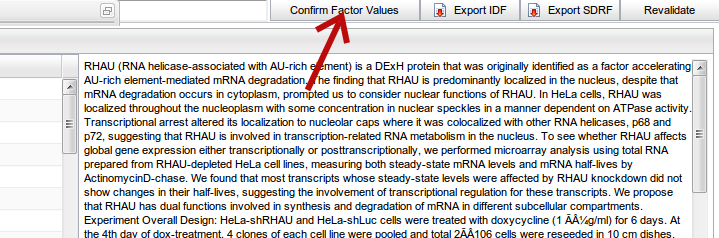
\includegraphics[width=17cm]{images/confirmfactorbutton}
\end{figure}



\begin{figure}[h]
\caption{Confirm factor value window}
\centering
\label{confirmfactorvalue}
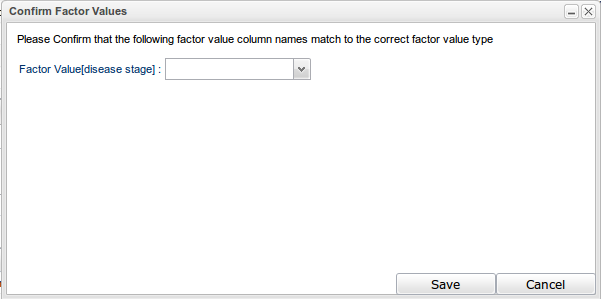
\includegraphics[width=12cm]{images/confirmfactorvalues}
\end{figure}

\section{Revalidation/Validation}
MageComet also has implementation of the Limpopo validators. A user can see all the of the errors by clicking on the Errors tab as shown in Figure \ref{errors}. 

In the errors tab, the user can selectively view errors, warnings, missing information, and revalidate the current MAGE-TAB documents after changes have been made.

\begin{figure}[h]
\caption{Errors button}
\centering
\label{errors}
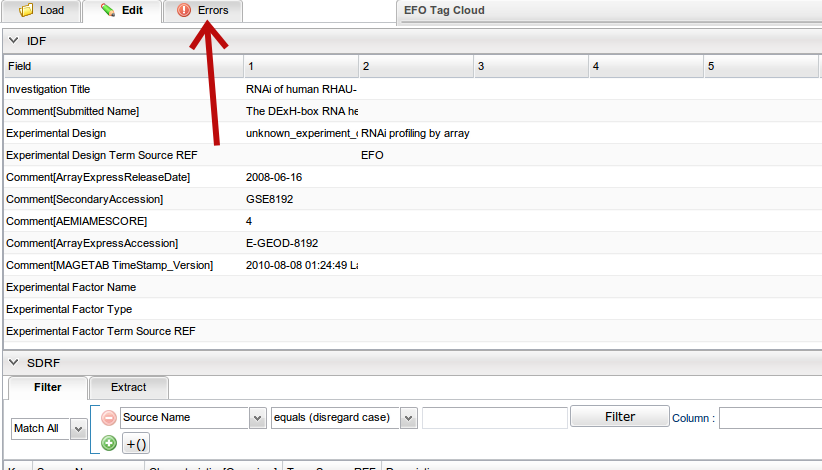
\includegraphics[width=17cm]{images/errors}
\end{figure}

\begin{figure}[h]
\caption{Errors tab}
\centering
\label{errorstab}
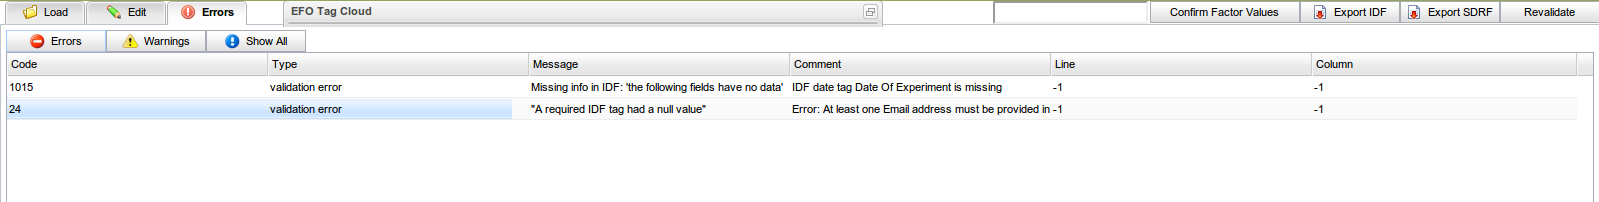
\includegraphics[width=17cm]{images/errors_tab}
\end{figure}

\newpage
\section{Exporting}
The final stage in editing is exporting the changes. To save a file locally, the user can click either "Export" button as designated by Figure \ref{export}.

\begin{figure}
\caption{Export buttons}
\centering
\label{export}
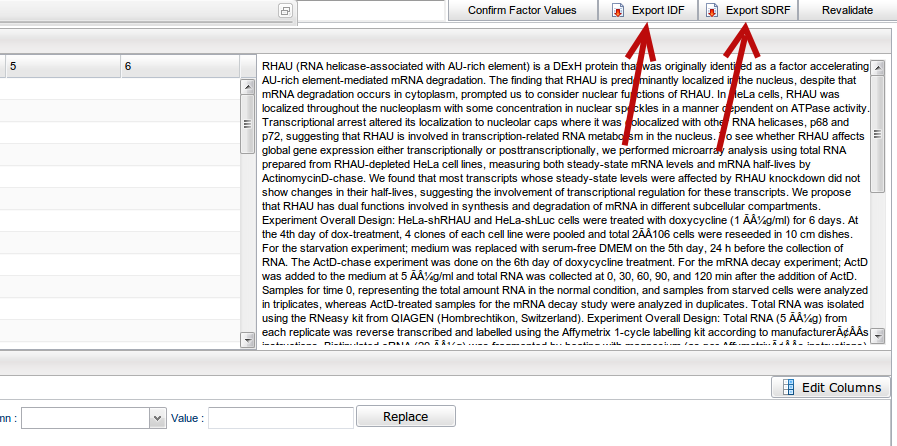
\includegraphics[width=17cm]{images/export}
\end{figure}




\end{document}
